\begin{python}
self.dashboard <= w.label('headline1', typo='headline1')
self.dashboard <= w.label('headline2', typo='headline2')
self.dashboard <= w.label('headline3', typo='headline3')
self.dashboard <= w.label('headline4', typo='headline4')
self.dashboard <= w.label('headline5', typo='headline5')
self.dashboard <= w.label('headline6', typo='headline6')
self.dashboard <= w.label('body1', typo='body1')
self.dashboard <= w.label('body2', typo='body2')
self.dashboard <= w.label('subtitle1', typo='subtitle1')
self.dashboard <= w.label('subtitle2', typo='subtitle2')
self.dashboard <= w.label('caption', typo='caption')
self.dashboard <= w.label('button', typo='button')
self.dashboard <= w.label('overline', typo='overline')
\end{python}

\begin{figure}[H]
\begin{centering}
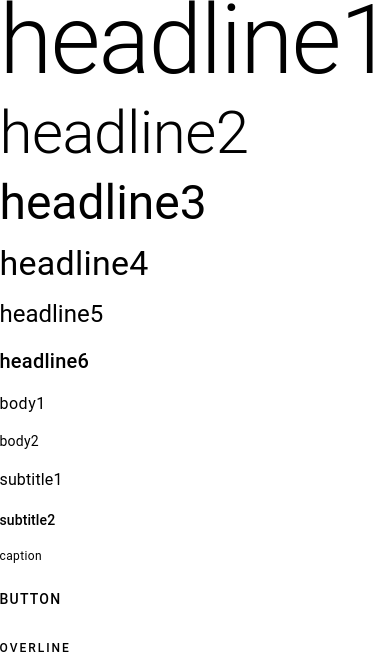
\includegraphics[scale=0.5]{Cap4/Figures/widgets/typography.png}
\par\end{centering}
\caption[Brython Radiant: Typography]{Brython Radiant: Default typography.}
\label{fig:radiant_typography}
\end{figure}